\documentclass[10pt,letterpaper]{article}

\usepackage[utf8]{inputenc}
\usepackage[T1]{fontenc}
\usepackage[letterpaper,margin=1.0in]{geometry}
\usepackage{authblk}
\usepackage{tabularx,booktabs}
\usepackage{multirow}
\usepackage{graphicx}
\usepackage{amsmath,amssymb}
\usepackage{placeins}
\usepackage{microtype}
\usepackage[labelfont=bf,font=small]{caption}
\captionsetup{skip=3pt}
\captionsetup[figure]{skip=6pt}
\usepackage[hidelinks]{hyperref}


% Compact float spacing to keep the body within the page limit.
\setlength{\textfloatsep}{6pt plus 2pt minus 2pt}
\setlength{\floatsep}{6pt plus 2pt minus 2pt}
\setlength{\intextsep}{8pt plus 2pt minus 2pt}
\usepackage{titlesec}
\linespread{0.93} % tighter leading so the body, including the Conclusion, ends on page 10
\AtBeginDocument{\setlength{\abovedisplayskip}{3pt plus 2pt}\setlength{\belowdisplayskip}{3pt plus 2pt}}
\titleformat*{\section}{\large\bfseries}
\titleformat*{\subsection}{\normalsize\bfseries}
\titlespacing*{\section}{0pt}{1.2ex plus 0.3ex minus 0.2ex}{0.7ex plus 0.2ex}
\titlespacing*{\subsection}{0pt}{1.0ex plus 0.3ex minus 0.2ex}{0.5ex plus 0.2ex}
\titlespacing*{\paragraph}{0pt}{1.2ex plus 0.3ex minus 0.2ex}{1em}

% Cross-references to the Appendix (supplementary.tex), prefix S-. The labels are stored in
% supplementary_labels.tex; regenerate it if the appendix numbering changes.
% Labels of supplementary_v6.tex for cross-references from manuscript_v6.tex (prefix S-).
% Generated from the compiled appendix; regenerate if the appendix numbering changes.
\newlabel{S-app:architecture}{{C}{6}{}{}{}}
\newlabel{S-app:data}{{A}{1}{}{}{}}
\newlabel{S-app:setting}{{B}{4}{}{}{}}
\newlabel{S-fig:detailed}{{S1}{7}{}{}{}}
\newlabel{S-fig:leadprio}{{S4}{29}{}{}{}}
\newlabel{S-sec:ablation42}{{F.3}{31}{}{}{}}
\newlabel{S-sec:ablation_phases}{{H.9}{43}{}{}{}}
\newlabel{S-sec:attribution}{{G}{33}{}{}{}}
\newlabel{S-sec:classification}{{F.1}{19}{}{}{}}
\newlabel{S-sec:encoder}{{C.1}{6}{}{}{}}
\newlabel{S-sec:evaluation}{{E}{14}{}{}{}}
\newlabel{S-sec:external_set}{{A.1}{3}{}{}{}}
\newlabel{S-sec:fixed_budget}{{H.2}{39}{}{}{}}
\newlabel{S-sec:generalization}{{G.7}{38}{}{}{}}
\newlabel{S-sec:leadprio_methods}{{E.1}{18}{}{}{}}
\newlabel{S-sec:leadprio}{{F.2}{27}{}{}{}}
\newlabel{S-sec:robustness}{{H}{39}{}{}{}}
\newlabel{S-sec:softedge}{{C.2}{8}{}{}{}}
\newlabel{S-sec:training}{{D}{10}{}{}{}}
\newlabel{S-tab:ablation42}{{S11}{33}{}{}{}}
\newlabel{S-tab:architecture}{{S2}{10}{}{}{}}
\newlabel{S-tab:baselines}{{S3}{17}{}{}{}}
\newlabel{S-tab:confusion}{{S9}{27}{}{}{}}
\newlabel{S-tab:data_stats}{{S1}{3}{}{}{}}
\newlabel{S-tab:paired}{{S4}{22}{}{}{}}
\newlabel{S-tab:random}{{S5}{24}{}{}{}}


\newcommand{\repourl}{\url{https://github.com/ashleyatmsft/gift}}

\begin{document}

% title page
\thispagestyle{empty}

\title{Graph-Informed Fusion for Inductive Drug-Target Interaction Prediction and Compound Prioritization in Lung Cancer}

\author[1,2]{Luis H. M. Torres}
\author[3]{Sumaiya Iqbal}
\author[1]{Ashley Mae Conard}
\affil[1]{\small Microsoft Research, Cambridge, MA, USA}
\affil[2]{\small Centre for Informatics and Systems of the University of Coimbra, Department of Informatics Engineering, Univ Coimbra, Coimbra, Portugal}
\affil[3]{\small Broad Institute of MIT and Harvard}


\date{}

\maketitle
\thispagestyle{empty}

\begin{abstract}
  Identifying compounds that act on disease-relevant proteins is central to drug discovery and repurposing, but experimentally testing every compound-target pair is impractical. Models that evaluate pairs independently do not exploit known relationships among compounds and proteins. Graph-based models capture these relationships, but extending their predictions to candidate compounds with few or no graph connections remains challenging.
To address these gaps, here we present \textbf{GIFT} (Graph-Informed Fusion for Target interaction prediction), a single inductive framework for both drug-target interaction (DTI) prediction and compound prioritization that ranks compounds for a target even when those compounds are absent from the interaction graph. GIFT combines three complementary modules. First, an edge-aware graph neural network is pretrained by contrastive learning, using hard negatives that share the compound or the protein of a true interaction, while a learnable soft-edge module proposes additional edges without directly supervising the proposed-edge scores. Second, an inductive per-node gate fuses these graph embeddings with representations learned from molecular and protein-sequence descriptors, so a prediction can be made when graph evidence is missing. Third, compound and protein nodes are randomly masked while the interaction classifier is trained, forcing it to predict interaction labels for nodes with and without graph connectivity.

We demonstrate the utility of GIFT using a lung cancer-focused knowledge graph integrating ChEMBL bioactivities, protein-protein interactions, and compound similarities. We evaluated GIFT against eight machine-learning and deep-learning baselines (random forest, GCN, GraphSAGE, GAT, DeepDTA, GraphDTA, DrugBAN, and the pretrained-representation model DTIAM) across 30 runs with different random seeds and data splits, excluding validation and test DTI edges from the message-passing graph. GIFT significantly outperformed all eight baselines (two-sided paired Wilcoxon tests, Holm-corrected) in mean PR-AUC, precision, and Matthews correlation coefficient (MCC) across three increasingly demanding benchmarks: (i) predicting held-out ChEMBL~35 interactions with random negative pairs ($p<10^{-5}$); (ii) identifying which targets the same test compounds act on using compound-matched negatives ($p<10^{-5}$); and (iii) predicting interactions recorded in ChEMBL~36 for 95 clinical-stage drugs outside the training graph ($p<10^{-7}$). These results demonstrate improved target identification and generalization beyond compounds represented during training.

The prediction advantage translated into improved compound prioritization: across 10 actionable driver kinases of non-small cell lung cancer, $4.8$ of GIFT's 10 highest-ranked drugs, on average, had known activity against the target, significantly more than DeepDTA, GraphDTA, DrugBAN, and DTIAM ($p<10^{-4}$). The top-ranked predictions included established clinically relevant lung cancer drug-target pairs, including ceritinib-ALK and dacomitinib-EGFR, demonstrating generalization to drugs outside the training graph. Demonstrated here for lung cancer, GIFT offers a reusable architecture that can be trained on compound-protein interaction data from other disease settings. By linking interaction prediction with target-specific compound ranking, GIFT provides a general framework for prioritizing candidates for more targeted experimental testing.


  \medskip
  \noindent\textbf{Code and data:} \repourl
\end{abstract}

\clearpage
\setcounter{page}{1}

% main text
\section{Introduction}
\label{sec:intro}
Drug discovery is a long and expensive process, often requiring more than a decade of development and carrying a substantial risk of failure \cite{hughes2011principles, paul2010improve}. 
Small-molecule drug discovery traditionally progresses through sequential and fragmented stages, including target identification, candidate compound identification and optimization, preclinical evaluation, and clinical testing \cite{hughes2011principles}. Drug repurposing can reduce development time and cost by identifying new therapeutic opportunities for approved or late-stage compounds \cite{pushpakom2019drug}. 
In both settings, identifying compounds that act on disease-relevant proteins can guide candidate selection. 
Because experimentally testing every compound-target pair is impractical, predicting drug-target interactions (DTIs) can help determine which compounds to test.
Lung cancer, the leading cause of cancer death, illustrates this need: many non-small cell lung cancers depend on oncogenic driver kinases such as EGFR, ALK, ROS1, and RET, and the clinical success of their inhibitors motivates systematic searches for compounds active at these and other disease-associated proteins \cite{herbst2018biology}.

DTI prediction methods differ in the information they use to score a compound-target pair. Random forests combine decision trees trained on predefined features to predict activity \cite{breiman2001random, svetnik2003random, mayr2018large}. Pairwise neural models learn compound and protein representations: DeepDTA uses convolutional networks to encode molecular structures written as SMILES strings and protein sequences \cite{ozturk2018deepdta}, whereas GraphDTA combines a graph neural network (GNN) over each compound's atoms and bonds with a convolutional protein-sequence encoder \cite{nguyen2021graphdta}. Both were developed for binding-affinity prediction. DrugBAN predicts binary interactions through bilinear attention between molecular substructures and protein-sequence features; its published framework also includes adaptation across different data distributions \cite{bai2023interpretable}. 
DTIAM combines compound and protein representations learned through large-scale pretraining on unlabeled molecules and protein sequences, using automated machine learning for downstream prediction \cite{lu2025dtiam}. These models can score compounds absent from the labeled training set, but do not explicitly aggregate information across a network of known compound-protein interactions and protein-protein relationships.

Interaction-network methods incorporate this broader information by connecting compounds and proteins through known activities, chemical similarities, and biological associations \cite{gaudelet2021utilizing, zhong2025knowledge, perdomoquinteiro2024knowledge}. Whereas the molecular graphs in GraphDTA and DrugBAN connect atoms within individual compounds, these networks connect different compounds and proteins. Applied to such networks, GCN combines normalized neighbor features \cite{kipf2017semi}, GraphSAGE samples and aggregates neighbor features \cite{hamilton2017inductive}, and GAT learns attention weights for neighboring nodes \cite{velickovic2018graph}. The resulting representations can be combined to predict compound-protein interactions. Their access to network information, however, depends on the available connections.
Compounds without known DTIs may still connect to similar compounds, but compounds without any connections have no compound-neighborhood information to aggregate. GraphSAGE can represent unseen nodes, but this does not supply missing interaction evidence. Graph structure learning offers a complementary approach by learning or refining connections during training \cite{zhu2021deep, jin2020graph, chen2020iterative, fatemi2021slaps}. Nevertheless, these connections remain model proposals rather than experimentally confirmed interactions.

These approaches leave two linked modeling challenges for compound prioritization: combining molecular information with interaction-network evidence when available, and making useful predictions when a candidate has no graph connections. Establishing whether a model meets these challenges raises a third challenge, its evaluation. Sparse activity measurements and uneven experimental coverage make it difficult to establish whether performance on well-studied compounds and proteins extends to less-studied candidates \cite{mayr2018large, pahikkala2015toward}. 
Treating unmeasured pairs as inactive can introduce incorrect negative labels, while class imbalance makes overall accuracy insufficient to assess recovery of active compounds. Evaluation can further obscure these limitations: random pair-level splits often place the same compounds and proteins in training and testing, and related chemical series can make performance appear stronger than it is on structurally different compounds \cite{pahikkala2015toward, mayr2018large}. 
For pretrained models, exclusion from labeled interaction training does not necessarily mean exclusion from pretraining. In network-based models, retaining held-out interactions as observed input edges reveals the very relationships being predicted \cite{kaufman2012leakage}. Finally, strong classification results across compound-target pairs do not establish that a model ranks active compounds highly for each individual target, which determines the usefulness of a short list for experimental testing \cite{pahikkala2015toward}. Together, these challenges motivate a framework that combines network and molecular information, explicitly trains for missing graph connections, and is assessed both on compounds outside the training graph and on target-specific candidate rankings.

\begin{figure}[t!]
\centering
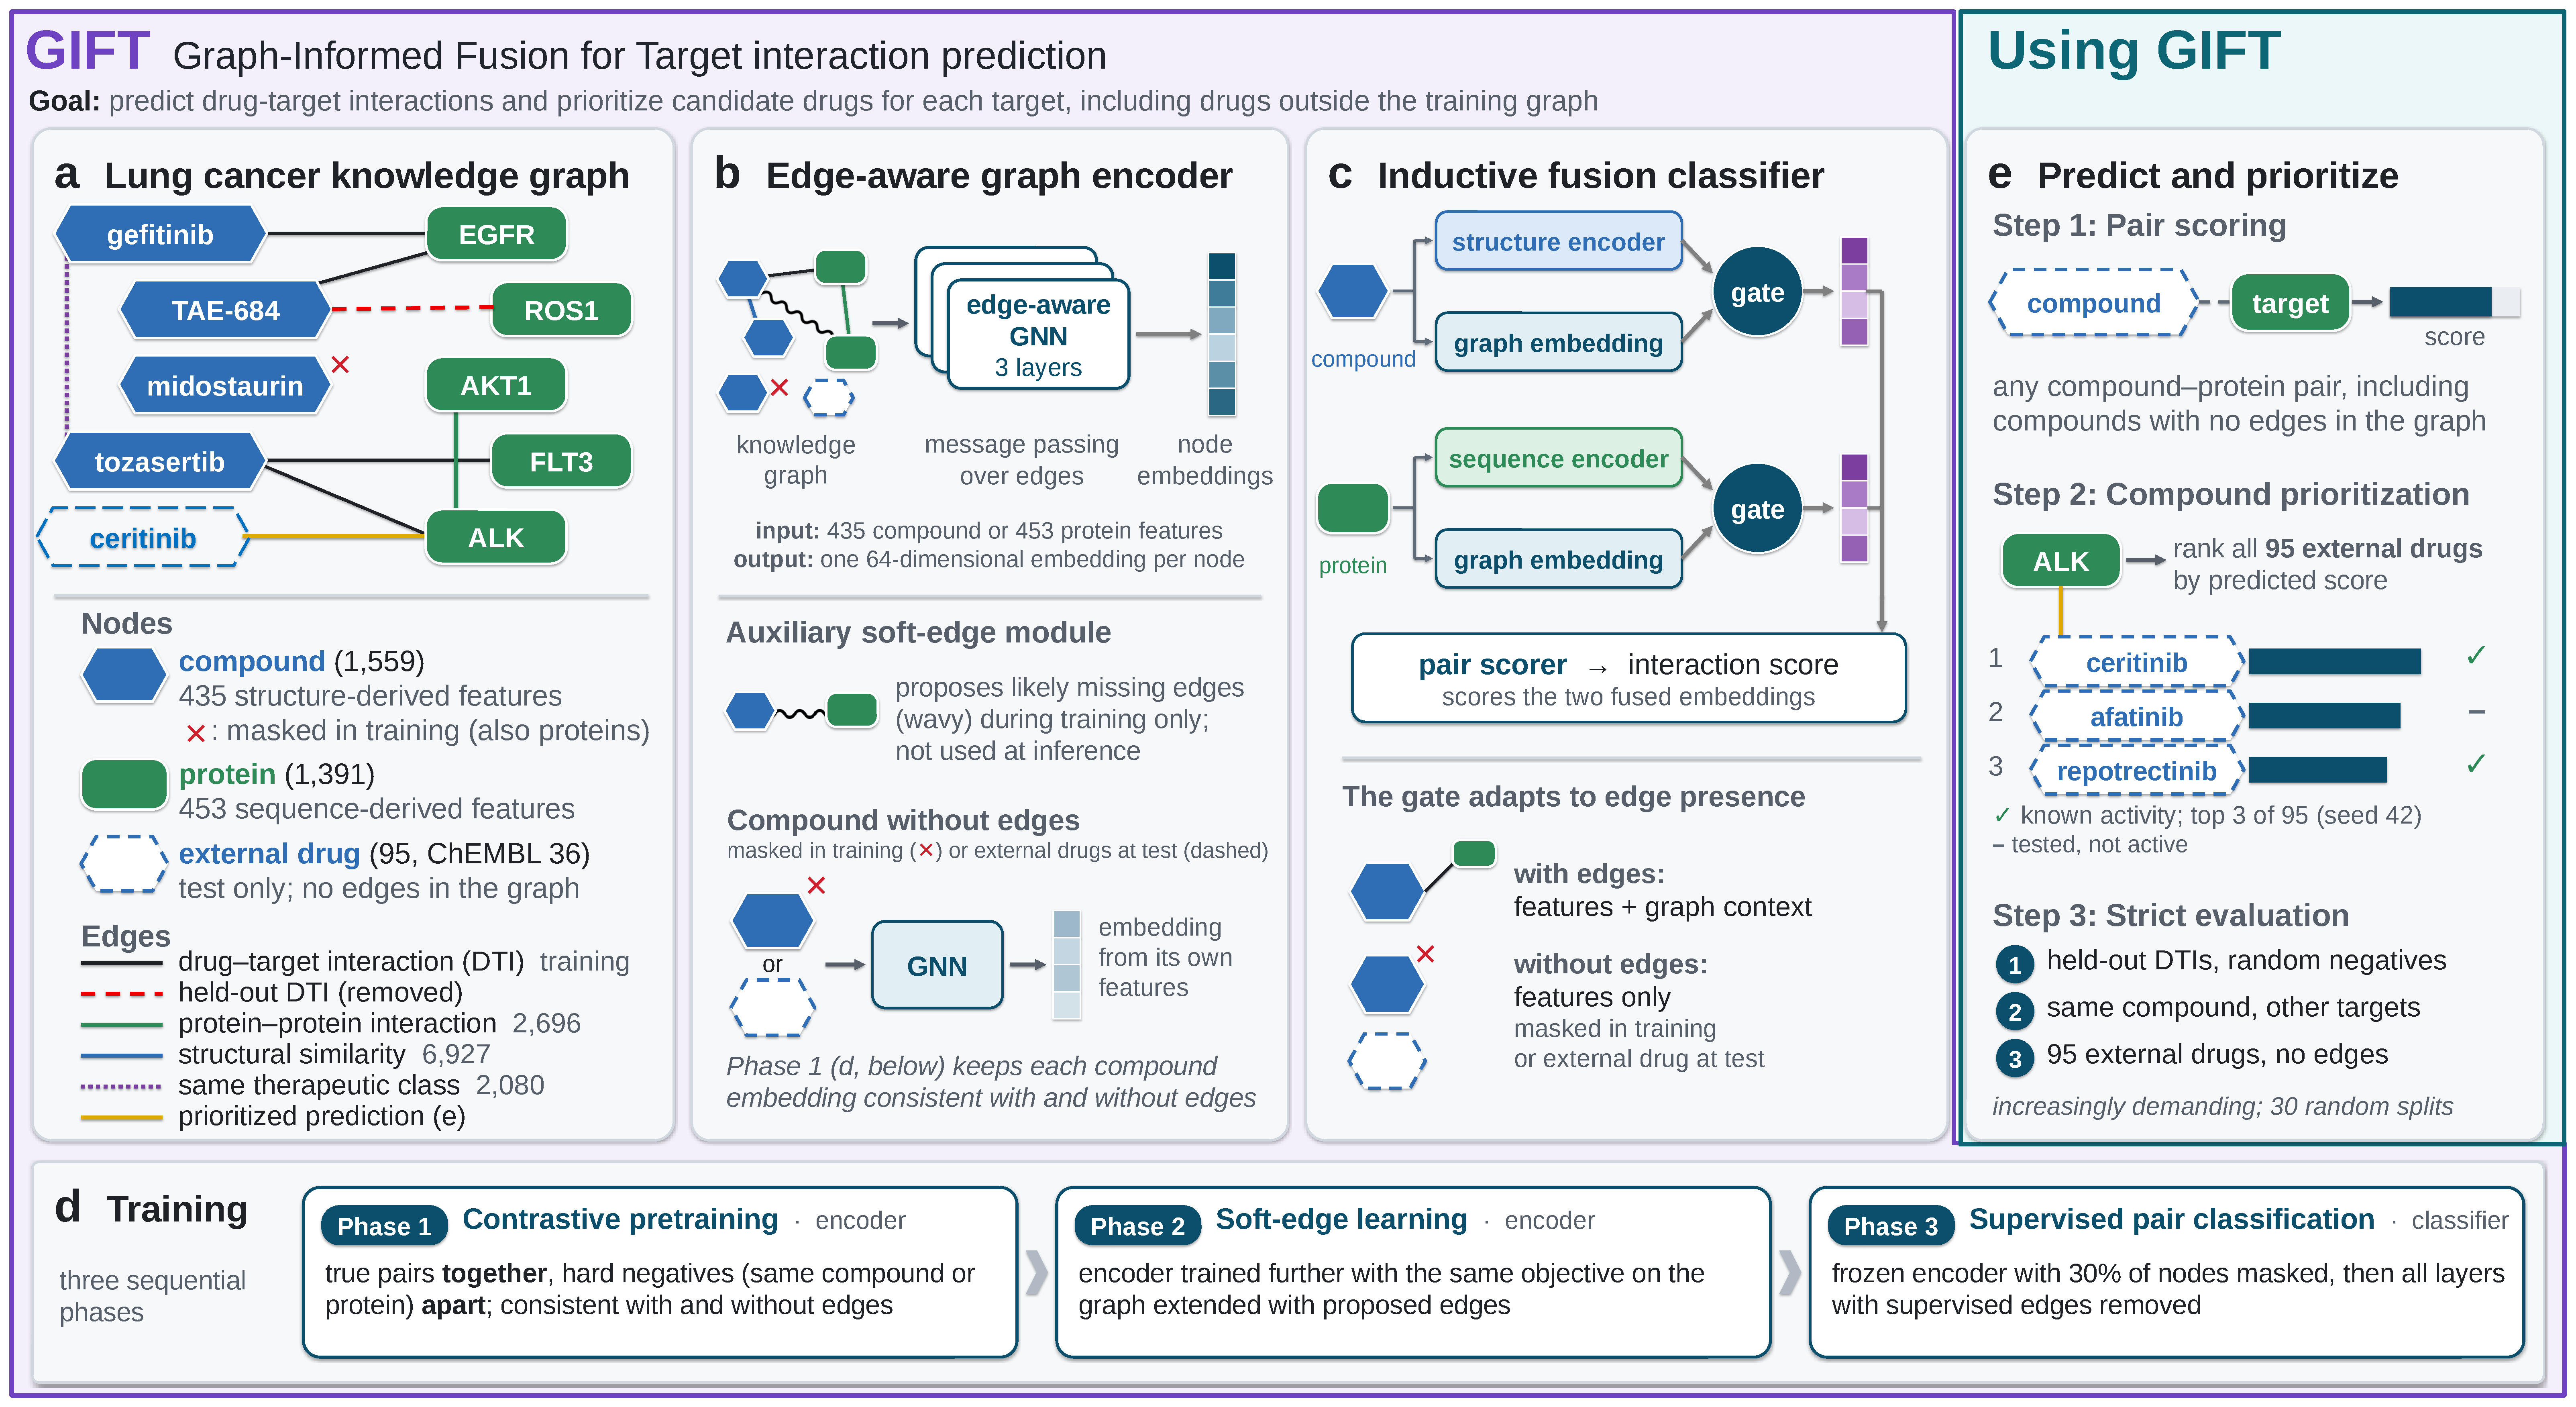
\includegraphics[width=\textwidth]{figs/architecture.pdf}
\caption{Overview of the GIFT framework. First, (a)~we construct a lung cancer knowledge graph that links compounds and proteins through training drug-target interactions (DTIs), protein-protein interactions, and compound similarity; held-out DTIs are removed, and the 95 external drugs enter without edges. Then, (b)~an edge-aware graph neural network embeds each node, including nodes without edges: training compounds whose edges are masked and, at test time only, the external drugs. Next, (c)~a gate fuses each node's feature encoding with its graph embedding, so that graph context enters only for nodes with edges, and a pair scorer outputs the interaction score. (d)~Training proceeds in three complementary phases (Section~\ref{sec:training}). Finally, in use, (e)~GIFT scores any compound-protein pair and ranks the external drugs for each target (ALK example from the run with seed 42). Shaded squares are embedding vectors (grey: from a compound's own features); bars in (e) are interaction scores.}
\label{fig:architecture}
\end{figure}

To combine interaction-network information with prediction for compounds lacking graph connections, we present GIFT (Graph-Informed Fusion for Target interaction prediction), a graph-based deep learning framework for DTI prediction and compound prioritization that is inductive, that is, it also scores compounds absent from the training graph, and we demonstrate it on lung cancer-associated targets as one application (Figure~\ref{fig:architecture}; detailed overview in Figure~\ref{S-fig:detailed}). The four main contributions are:

(i)~an edge-aware GNN encoder over a lung cancer knowledge graph that integrates ChEMBL bioactivity data with STRING protein-protein interactions and compound-compound relationships, in which edge attributes weight the information passed between connected nodes, and which is pretrained contrastively with hard negatives that share the compound or the protein of a known interaction and with consistency losses between connected and isolated compound representations (Figure~\ref{fig:architecture}a,b,d), whose node embeddings are passed to
(ii)~an inductive fusion classifier that combines them with descriptor-based compound and protein encoders through a gate that uses both representations and a binary flag indicating whether the node has any edges; removing the edges of selected nodes during training teaches it to score compounds with or without graph connections (Figure~\ref{fig:architecture}c,d);
(iii)~during encoder training, an auxiliary soft-edge structure-learning module for the heterogeneous graph, which proposes compound-protein, compound-compound, and protein-protein edges with type-specific scorers, is optimized through contrastive training rather than direct supervision of proposed-edge labels, and is not used at inference (Figure~\ref{fig:architecture}b,d); and, to assess GIFT,
(iv)~a leakage-free evaluation that separates interaction prediction from target-level compound prioritization: we compare GIFT with random forest, standard GNN, pairwise DTI deep-learning, and pretrained-representation baselines on three DTI benchmarks (held-out ChEMBL~35 interactions with random negatives, the same interactions with compound-matched negatives, and interactions of drugs outside the training graph) from which all validation and test DTIs are removed before training, and we rank 95 clinical-stage drugs for each target and compare these rankings with a family-level ranking to assess whether they distinguish between targets (Figure~\ref{fig:architecture}e).

Across three DTI benchmarks and 30 runs, GIFT achieves the highest mean PR-AUC, precision, and MCC among the nine methods (two-sided paired Wilcoxon tests, Holm-corrected $p<10^{-5}$ against each baseline, Table~\ref{tab:main}).
On the external benchmark, its 100 highest-scoring compound-target pairs include 81.5 known actives on average, compared with 69.2 for GraphDTA, the next-best method (Appendix~\ref{S-sec:robustness}).
When ranking 95 clinical-stage drugs separately for ten driver kinases relevant to non-small cell lung cancer, GIFT recovers 4.8 known actives among the ten highest-ranked drugs, compared with 4.3 for DTIAM, the strongest of the four DTI baselines for this ranking task (Holm-corrected $p<10^{-4}$), and 1.6 expected at random.
Although discrimination between individual driver kinases remains limited, GIFT enriches candidate shortlists for known kinase-active compounds, supporting their prioritization for experimental follow-up.

\section{Methods}
\label{sec:methods}
GIFT predicts, for a compound $c$ and a protein $p$, an interaction score $\hat{y}_{cp}\in(0,1)$, trained to separate active from inactive pairs, and ranks candidate compounds for each target by this score (Figure~\ref{fig:architecture}). It has three components: an edge-aware GNN encoder that computes node embeddings from the knowledge graph (Sections~\ref{sec:graph},~\ref{sec:encoder}); a soft-edge module that proposes additional edges to the encoder during representation learning only (Section~\ref{sec:softedge}); and an inductive fusion classifier that combines graph embeddings with descriptor encodings and scores each pair (Section~\ref{sec:fusion}). The encoder is pretrained contrastively (Phases~1 and~2, Section~\ref{sec:training}), and the classifier is trained on the frozen encoder and then fine-tuned jointly with it (Phase~3; Section~\ref{sec:training}). At inference, only the encoder, applied to the training graph, and the classifier are used, allowing compounds without edges to be scored from their descriptors. We share details of the data and features (Appendices~\ref{S-app:data} and~\ref{S-app:setting}), the architecture (Appendix~\ref{S-app:architecture}), the training procedure and its hyperparameters (Appendix~\ref{S-sec:training}, Table~\ref{S-tab:architecture}), and the evaluation protocol and baseline configurations (Appendix~\ref{S-sec:evaluation}, Table~\ref{S-tab:baselines}) to enable reproducibility and consistent evaluation.



\subsection{Problem setting: a lung cancer knowledge graph of compounds and proteins}
\label{sec:graph}
To give the model both molecular information and the network of known relationships, compounds and proteins are nodes of a knowledge graph. The graph was constructed from ChEMBL~35 \cite{zdrazil2024chembl} for the lung cancer domain (Appendix~\ref{S-app:data}, Table~\ref{S-tab:data_stats}). It contains $|\mathcal{V}_c|=1{,}559$ compounds and $|\mathcal{V}_p|=1{,}391$ proteins. A compound-protein pair is a DTI, or interaction, if its median pChEMBL over all ChEMBL records is $\geq 5$ (10~$\mu$M or better), which yields 2,865 interactions; the remaining 11,588 tested pairs are neither edges nor positives and are excluded from the evaluation negatives. The graph also contains 2,696 STRING protein-protein interactions \cite{szklarczyk2023string} and 9,007 compound-compound edges (6,927 Tanimoto-similarity edges of Morgan fingerprints and 2,080 therapeutic-class edges). Compounds are described by 435 structure-derived features (molecular descriptors, Morgan fingerprint, MACCS keys) and proteins by 453 sequence-derived features (amino-acid and dipeptide composition, physicochemical and complexity statistics); no feature is derived from interaction records. Each edge $(i,j)$ has a two-dimensional attribute $e_{ij}$ encoding its strength (pChEMBL, STRING confidence, or Tanimoto similarity) and its type or evidence level. DTI prediction is link prediction on this graph: given a compound $c$ and a protein $p$, predict $\hat{y}_{cp}\in(0,1)$. Throughout, a \emph{pair} is any compound-protein combination, whether or not it interacts, and a \emph{DTI} is a pair that does; \emph{compound} refers to any small molecule, and \emph{drug} is reserved for the clinical-stage compounds of the external set.

To test generalization to compounds absent from the graph, we use an external set of 95 clinical-stage drugs annotated in ChEMBL~36 with a lung cancer indication (8 approved for lung cancer and 87 in clinical trials for it), selected without regard to their similarity to the graph compounds, which provides 3,243 interactions at 690 graph proteins under the same activity definition (Appendix~\ref{S-sec:external_set}). Since 96.0\% of these interactions are supported by records in ChEMBL~35 or earlier, the set measures generalization to compounds outside the graph rather than to future measurements (a retrospective analysis of the interactions first reported later is in Appendix~\ref{S-sec:robustness}). The drugs are structurally distant from the training compounds (median nearest-neighbor Tanimoto similarity 0.24, compared with 0.50 for the ChEMBL~35 test compounds of the run with seed 42) and are added to the graph as isolated nodes.

\subsection{Edge-aware graph encoder: learning compound and protein representations}
\label{sec:encoder}
To learn compound and protein representations that account for the type and strength of their graph connections, node features are placed in disjoint type-specific blocks of an 888-dimensional input $H^{(0)}$. Throughout, node and edge vectors are row vectors, and every linear map includes a bias. Three edge-gated convolution layers ($888\to128\to128\to64$) compute
\begin{equation}
\tilde{H}^{(\ell)}_i = \alpha_{ii}\big(H^{(\ell-1)}_i W^{(\ell)} + b^{(\ell)}\big) + \sum_{j\in\mathcal{N}(i)} \alpha_{ij}\big(H^{(\ell-1)}_j W^{(\ell)} + b^{(\ell)}\big)\odot\sigma\!\big(e_{ij} W_e^{(\ell)} + b_e^{(\ell)}\big),
\qquad \alpha_{ij} = D_{ii}^{-1/2} D_{jj}^{-1/2},
\label{eq:conv}
\end{equation}
where $D_{ii}=1+|\mathcal{N}(i)|$ counts the self-loop, with LayerNorm and ReLU after layers 1 and 2 and edge dropout of 0.15 during training. The sigmoid gate rescales each channel of a neighbor's message according to its edge attributes, a relation- and evidence-dependent weighting with a single set of node weights \cite{schlichtkrull2018modeling}. For a node without edges, $D_{vv}=1$ and $\tilde{H}^{(\ell)}_v=H^{(\ell-1)}_vW^{(\ell)}+b^{(\ell)}$ in every layer, making its embedding a deterministic function of its own features. The node embedding $z_v\in\mathbb{R}^{64}$ combines a type-specific projection of $H^{(3)}_v$ and a learnably weighted skip connection from the input features (Appendix~\ref{S-sec:encoder}).

\subsection{Soft-edge module: proposing missing edges during representation learning}
\label{sec:softedge}
As fewer than 0.2\% of compound-protein pairs are known interactions, the neighborhoods that the encoder aggregates are sparse; to expose it to plausible unobserved relationships, the soft-edge module learns which compound-protein, compound-compound, and protein-protein pairs to connect so as to reduce the contrastive loss of the encoder. It scores every candidate pair of three relation types: all 2.17 million compound-protein pairs and all unordered compound-compound and protein-protein pairs, without filtering against observed edges and without using any label. From the layer-2 activations $U=H^{(2)}$, compound queries $Q=\mathrm{LN}(U_cW_Q+b_Q)$ and protein keys $K=\mathrm{LN}(U_pW_K+b_K)$ are split into $H=4$ heads, and each head scores a pair with its own MLP:
\begin{equation}
S_{cp} = \sigma\!\Big(\frac{1}{\tau}\sum_{h=1}^{H} w_h\, \mathrm{MLP}^{(h)}\big([Q_c^{(h)}\,\|\,K_p^{(h)}]\big)\Big),\qquad w=\mathrm{softmax}(\omega),
\label{eq:softedge}
\end{equation}
with a learned temperature $\tau$. Compound-compound and protein-protein pairs are scored analogously with separate parameters. At epoch $t$ of Phase~2, the module keeps the top $k_{\text{CP}}(t)=1000(t+1)$ compound-protein and $k_{\text{CC}}(t)=k_{\text{PP}}(t)=100(t+1)$ homogeneous pairs, allowing the encoder to see progressively larger neighborhoods (200,000 compound-protein proposals at the last epoch). Selected pairs are added in both directions to the input of layer~3 with attributes $(S_{ij},S_{ij})$, such that in Eq.~\eqref{eq:conv} each channel of a proposed message is a monotone function of its score.

The top-$k$ selection passes no gradient; the module is trained only through the edge gates of the selected pairs by the Phase~2 contrastive objective; no interaction label is a target for the scores, and at inference, embeddings are computed without proposed edges (Appendix~\ref{S-sec:softedge}).

\subsection{Inductive fusion classifier: scoring pairs with or without graph connections}
\label{sec:fusion}
Because the external drugs and masked training nodes have no edges, the classifier must score a pair from descriptors alone when graph evidence is missing and add graph context when it is available. Descriptor encoders $T_c$ and $T_p$ ($888\to384\to192$) map every node to $f_v$, whether or not it has edges. Graph embeddings are projected to $g_v=\mathrm{LN}(z_vW_g+b_g)\in\mathbb{R}^{192}$, and a per-dimension gate determines how much of $g_v$ is added:
\begin{equation}
h_v = f_v + \sigma\!\big(\mathrm{MLP}([f_v\,\|\,g_v\,\|\,\kappa_v])\big)\odot g_v,
\label{eq:gate}
\end{equation}
where $\kappa_v\in\{0,1\}$ indicates whether the node has at least one edge in the current forward pass. Masked nodes and external drugs have $\kappa_v=0$. Setting $\kappa_v=0$ does not switch off the second pathway: for a node without edges, the encoder still computes $z_v$, and hence $g_v$, from the node's own features (Section~\ref{sec:encoder}), so the gated term adds a second descriptor-derived representation rather than graph evidence. The flag allows the gate to weight $g_v$ differently depending on whether it carries neighborhood information. The gate receives only this binary flag rather than the node degree, which prevents the classifier from using the number of known interactions as a shortcut. A pair is scored as $\hat{y}_{cp}=\sigma\big(\mathrm{MLP}([h_c\,\|\,h_p\,\|\,h_c\odot h_p\,\|\,|h_c-h_p|]) + h_cBh_p^{\top} + b_B\big)$ with a learned bilinear form $B$ and bias $b_B$. The model has 1.9 million parameters.

\subsection{Three-phase training: from contrastive representation learning to pair classification}
\label{sec:training}
Training proceeds from representation learning to prediction: Phases~1 and~2 train the encoder to place interacting pairs close together in embedding space, and Phase~3 trains the classifier, first alone and then jointly with the encoder, to predict interaction labels. Every phase uses the training graph, whose only compound-protein edges are the training interactions, and negatives exclude both training interactions and pairs of the evaluation reserve (Section~\ref{sec:evaluation}). Full specifications are given in Appendix~\ref{S-sec:training}.

\paragraph{Phase 1: contrastive pretraining}
A pair is embedded as $u_{cp}=[\hat{z}_c\|\hat{z}_p]/\|[\hat{z}_c\|\hat{z}_p]\|$ with $\hat{z}=z/\|z\|$. For each anchor interaction $a=(c,p)$ in a batch $\mathcal{B}$ of 64, candidate negatives are 50 eligible pairs $(c,p')$, 50 eligible pairs $(c',p)$, and up to 30 random pairs; the negative set $\mathcal{N}_a$ contains the 7 candidates most similar to the anchor and 3 random ones, mined online \cite{schroff2015facenet, hermans2017defense}. As most candidates share the compound or the protein of the anchor, the encoder must separate a compound's targets from its non-targets and a protein's ligands from its non-ligands. With a pool $\mathcal{P}$ of other training interactions, the loss is
\begin{equation}
\mathcal{L}_{\text{tri}} = \frac{1}{|\mathcal{B}|}\sum_{a\in\mathcal{B}} \max\!\Big\{\epsilon,\ \gamma + \frac{1}{|\mathcal{N}_a|}\sum_{n\in\mathcal{N}_a} \langle u_a,u_n\rangle - \frac{1}{|\mathcal{P}|}\sum_{q\in\mathcal{P}} \langle u_a,u_q\rangle \Big\},
\label{eq:triplet}
\end{equation}
with margin $\gamma=2$, floor $\epsilon=10^{-4}$, and the cosine similarity $\langle u_a,u_n\rangle$ of unit-norm pair embeddings; it gathers interacting pairs into a common region of the pair space. Consistency terms align the embeddings with those of a second pass under resampled dropout, and isolation terms align each compound, and its training interactions, with a third pass in which up to 20\% of the compounds are isolated from the graph; since an isolated compound's embedding depends only on its descriptors, these terms pull graph-based embeddings toward the representation of compounds outside the graph.

\paragraph{Phase 2: soft-edge contrastive learning}
The encoder and the soft-edge module are trained jointly for 200 epochs with $\mathcal{L}_{\text{tri}}$ and an $L_2$ penalty on the compound-protein scorer, on the observed graph extended with the proposed edges.

\paragraph{Phase 3: supervised pair classification}
In Phase~3a, the encoder is frozen and the fusion classifier is trained with binary cross-entropy on all training interactions and one freshly sampled negative per positive, while in every epoch 30\% of the compounds and, independently, 30\% of the proteins are masked by removing all their edges, enabling the gate to learn when graph evidence is available. In Phase~3b, the encoder and the classifier are fine-tuned jointly; since every training interaction is also a graph edge, each step removes the edges of the 30\% of training interactions used as supervision targets, preventing the encoder from learning that an observed edge implies a positive label. Both phases select checkpoints on the mean validation-set ROC-AUC with the validation compounds connected to and isolated from the graph.

\subsection{Leakage-free evaluation protocol for interaction prediction and compound prioritization}
\label{sec:evaluation}
The evaluation tests whether GIFT generalizes beyond the interactions and compounds it was trained on, without any held-out information reaching the model. It comprises leakage-free splits and negatives, three DTI benchmarks of increasing difficulty, eight baselines trained under the same protocol, target-level rankings of the external drugs for compound prioritization, and a paired statistical comparison across runs.

To prevent leakage, the data are split before any training. In each of 30 runs (seeds 42-71), the 14,453 tested pairs are split at random 70/15/15 with the seed of the run and restricted to interactions (2,020, 402, and 443 in the run with seed 42). The validation set is used only for checkpoint selection, and the test set only for evaluation (benchmarks 1 and 2); together, we call them the \emph{held-out} interactions, and the external set (benchmark 3) is evaluated separately. All held-out interactions are removed from the graph before training, in both directions. A fixed random 20\% of all compound-protein pairs is reserved before training: evaluation negatives are drawn only from this reserve and exclude every tested pair, whereas training negatives of every model are drawn from the remaining 80\%. Evaluation negatives are therefore never used in training; held-out positives are not excluded from training negatives and are drawn at their base rate ($<$0.04\%), which can only lower their scores (Appendix~\ref{S-sec:robustness}).

Three DTI benchmarks of increasing difficulty are built from these splits. The first, \emph{ChEMBL~35 with random negatives} (1), tests the test-set interactions against five random negatives per positive, drawn from compounds with at least one interaction, as in standard DTI benchmarks. The second, \emph{ChEMBL~35 with compound-matched negatives} (2), tests the same positives against $5n_c$ negatives involving each test compound with $n_c$ positives, such that whether a compound is active carries no information and the task reduces to identifying its targets. The third, \emph{external compounds} (3), tests the 3,243 ChEMBL~36 interactions of the 95 external drugs against 15,646 negatives of the same drugs without any ChEMBL~36 record. Since 79\% to 90\% of the ChEMBL~35 test compounds have other interactions in the training set, benchmarks (1) and (2) mainly test the prediction of additional targets for known compounds, whereas benchmark (3) tests compounds absent from the graph. Scores are not calibrated, so a score above 0.5 is not a probability of confirmed activity. Because experimental follow-up depends on how candidates are ranked, the threshold-independent ranking metrics and the number of known actives recovered at a fixed candidate budget are the most practically relevant measures; classification metrics at a fixed threshold of 0.5, applied to every model, complement them, and a validation-chosen threshold gives the same ranking of methods (Appendix~\ref{S-sec:fixed_budget}). Ranking performance is measured by the ROC-AUC, the PR-AUC, and the per-target ROC-AUC (mean over targets with both classes, which cannot be raised by ranking frequently tested targets first), and classification at the threshold by precision, recall, MCC, and error counts. As interactions are a minority class, PR-AUC among the ranking metrics and precision and MCC among the classification metrics are the most informative \cite{saito2015precision, chicco2020advantages}.

GIFT is compared with eight baselines trained under the same protocol. The random forest (scikit-learn defaults) uses the 888 standardized descriptors of each pair; GCN, GraphSAGE, and GAT use a two-layer encoder ($888\to128\to64$) on the same training graph and features with a dot-product decoder; and DeepDTA, GraphDTA (GIN variant), and DrugBAN (official implementation) use their standard published configurations. All these baselines are trained from scratch in every run on the same training interactions of the knowledge graph as GIFT, with the same negative sampling rule, validation set, selection criterion, and split, without per-run hyperparameter search (Appendix~\ref{S-sec:evaluation}). DTIAM (official implementation) keeps its pretrained compound (BerMol) and protein (ESM-2) encoders frozen, as designed, and its interaction head is trained from scratch in every run under the same protocol.

Beyond these benchmarks, compound prioritization is evaluated with target-level rankings. For each target, the 95 external drugs are ranked by $\hat{y}_{cp}$ for two target sets fixed before any ranking was inspected: the 252 targets with at least five known actives, and the ten actionable driver kinases of non-small cell lung cancer in the graph (EGFR, ALK, ROS1, RET, MET, ERBB2, BRAF, NTRK1-3). Rankings are assessed by the ROC-AUC over the 95 drugs and the number of known actives among the 10 top-ranked drugs, and target specificity by comparison with a family ranking, which applies one ranking to every target of a family (the mean score over all kinases for a kinase target, or over all other proteins otherwise), and a global ranking (the mean score over all proteins) (Appendix~\ref{S-sec:leadprio_methods}). The three benchmarks thus evaluate DTI prediction, and these rankings evaluate compound prioritization.

Finally, the methods are compared statistically across runs. Every method is trained and evaluated once in each of the 30 runs, which differ in data split and initialization. The mean $\pm$ standard deviation across runs in the tables describes run-to-run variability, not the precision of a comparison. Methods are therefore compared run by run: the within-run difference between GIFT and a baseline (signed so that a positive value favors GIFT) is summarized by its mean and a 95\% percentile bootstrap confidence interval (10,000 resamples of the runs) and tested with the two-sided Wilcoxon signed-rank test, with $p$-values Holm-corrected within each family of comparisons: the eight baselines for each benchmark and metric (Table~\ref{tab:main}; differences and confidence intervals in Table~\ref{S-tab:paired}), the four DTI baselines for each driver-kinase shortlist metric (Table~\ref{tab:leadprio_baselines}), and the 40 kinase-baseline pairs of the per-kinase comparison (Table~\ref{tab:leadprio_kinases}, Figure~\ref{fig:toppicks}b). Unless stated otherwise, reported $p$-values are Holm-corrected. Rankings are compared within a run with the two-sided paired Wilcoxon test over targets, and ablation $p$-values are uncorrected and exploratory.

%
\section{Results}
\label{sec:results}
We evaluate GIFT on two tasks: predicting compound-target interactions and prioritizing compounds for individual targets. We first compare GIFT with eight baselines on held-out interactions using random and compound-matched negatives, and on drugs outside the training graph (Section~\ref{sec:classification}). We then examine whether GIFT ranks known actives highly among 95 clinical-stage drugs across 252 targets and ten driver kinases relevant to non-small cell lung cancer, and whether the driver-kinase rankings distinguish individual kinases or primarily reflect activity shared across the family (Section~\ref{sec:leadprio}). Unless otherwise stated, results are reported as mean $\pm$ standard deviation over 30 runs, each with its own data split, and differences between methods as mean paired differences with 95\% confidence intervals and Holm-corrected two-sided $p$-values (Section~\ref{sec:evaluation}). Complete classification results are provided (Appendix~\ref{S-sec:classification}, Tables~\ref{S-tab:random}-\ref{S-tab:confusion}).

\begin{table}[t!]
\centering
\caption{Classification on the three benchmarks (fixed threshold 0.5). Values are mean $\pm$ standard deviation over 30 runs, each with its own data split, and describe run-to-run variability; confidence intervals for the differences between methods are in Table~\ref{S-tab:paired}. FP: false positives; total errors: false positives plus false negatives. Best mean per row in bold. $^{\dagger}$Frozen pretrained compound and protein encoders; interaction head trained in every run. Per-run comparisons and complete confusion matrices are in Tables~\ref{S-tab:random}-\ref{S-tab:confusion}.}
\label{tab:main}
\resizebox{\textwidth}{!}{%
\begin{tabular}{l c c c c c c c c c}
\toprule
 & & & \multicolumn{3}{c}{\textbf{Standard GNN}} & \multicolumn{4}{c}{\textbf{DTI models}} \\
\cmidrule(lr){4-6}\cmidrule(lr){7-10}
\textbf{Metric} & \textbf{GIFT} & \textbf{RF} & \textbf{GCN} & \textbf{SAGE} & \textbf{GAT} & \textbf{DeepDTA} & \textbf{GraphDTA} & \textbf{DrugBAN} & \textbf{DTIAM}$^{\dagger}$ \\
\midrule
\multicolumn{10}{l}{\textit{ChEMBL~35, random negatives}} \\
PR-AUC $\uparrow$ & \textbf{0.907$\pm$0.010} & 0.827$\pm$0.013 & 0.658$\pm$0.034 & 0.655$\pm$0.035 & 0.532$\pm$0.046 & 0.886$\pm$0.026 & 0.858$\pm$0.022 & 0.789$\pm$0.042 & 0.854$\pm$0.014 \\
MCC $\uparrow$ & \textbf{0.818$\pm$0.019} & 0.512$\pm$0.015 & 0.540$\pm$0.030 & 0.634$\pm$0.024 & 0.480$\pm$0.067 & 0.716$\pm$0.043 & 0.723$\pm$0.036 & 0.608$\pm$0.081 & 0.519$\pm$0.023 \\
Precision $\uparrow$ & \textbf{0.859$\pm$0.032} & 0.413$\pm$0.012 & 0.459$\pm$0.035 & 0.614$\pm$0.038 & 0.398$\pm$0.052 & 0.662$\pm$0.065 & 0.716$\pm$0.066 & 0.528$\pm$0.099 & 0.412$\pm$0.023 \\
F1 $\uparrow$ & \textbf{0.848$\pm$0.016} & 0.572$\pm$0.012 & 0.604$\pm$0.028 & 0.696$\pm$0.021 & 0.550$\pm$0.053 & 0.760$\pm$0.039 & 0.769$\pm$0.031 & 0.661$\pm$0.075 & 0.574$\pm$0.021 \\
ROC-AUC $\uparrow$ & 0.962$\pm$0.005 & 0.939$\pm$0.006 & 0.904$\pm$0.010 & 0.911$\pm$0.008 & 0.882$\pm$0.016 & \textbf{0.963$\pm$0.006} & 0.950$\pm$0.007 & 0.943$\pm$0.012 & 0.949$\pm$0.006 \\
Per-target ROC-AUC $\uparrow$ & \textbf{0.950$\pm$0.013} & 0.930$\pm$0.013 & 0.906$\pm$0.018 & 0.914$\pm$0.015 & 0.881$\pm$0.019 & 0.946$\pm$0.013 & 0.936$\pm$0.016 & 0.925$\pm$0.018 & 0.938$\pm$0.012 \\
Recall $\uparrow$ & 0.838$\pm$0.023 & 0.931$\pm$0.013 & 0.889$\pm$0.021 & 0.805$\pm$0.024 & 0.905$\pm$0.021 & 0.898$\pm$0.021 & 0.836$\pm$0.029 & 0.911$\pm$0.035 & \textbf{0.948$\pm$0.013} \\
FP $\downarrow$ & \textbf{59.8$\pm$16.2} & 572.4$\pm$37.0 & 458.5$\pm$73.9 & 221.4$\pm$39.5 & 616.3$\pm$212.9 & 204.7$\pm$66.8 & 149.0$\pm$55.1 & 386.5$\pm$190.4 & 586.7$\pm$63.5 \\
Total errors $\downarrow$ & \textbf{129.9$\pm$14.1} & 602.2$\pm$36.8 & 506.5$\pm$69.2 & 305.4$\pm$35.1 & 657.2$\pm$205.2 & 248.9$\pm$61.3 & 219.7$\pm$46.9 & 425.2$\pm$180.1 & 609.3$\pm$60.7 \\
\midrule
\multicolumn{10}{l}{\textit{ChEMBL~35, compound-matched negatives}} \\
PR-AUC $\uparrow$ & \textbf{0.776$\pm$0.026} & 0.466$\pm$0.034 & 0.324$\pm$0.053 & 0.327$\pm$0.048 & 0.296$\pm$0.052 & 0.727$\pm$0.091 & 0.621$\pm$0.056 & 0.354$\pm$0.086 & 0.581$\pm$0.025 \\
MCC $\uparrow$ & \textbf{0.564$\pm$0.038} & 0.095$\pm$0.012 & 0.248$\pm$0.049 & 0.268$\pm$0.045 & 0.174$\pm$0.042 & 0.470$\pm$0.102 & 0.381$\pm$0.078 & 0.206$\pm$0.059 & 0.199$\pm$0.022 \\
Precision $\uparrow$ & \textbf{0.516$\pm$0.046} & 0.189$\pm$0.004 & 0.249$\pm$0.025 & 0.275$\pm$0.029 & 0.215$\pm$0.016 & 0.405$\pm$0.083 & 0.349$\pm$0.067 & 0.228$\pm$0.028 & 0.217$\pm$0.009 \\
F1 $\uparrow$ & \textbf{0.637$\pm$0.033} & 0.314$\pm$0.006 & 0.388$\pm$0.030 & 0.409$\pm$0.031 & 0.348$\pm$0.020 & 0.552$\pm$0.081 & 0.488$\pm$0.062 & 0.364$\pm$0.033 & 0.353$\pm$0.011 \\
ROC-AUC $\uparrow$ & \textbf{0.899$\pm$0.010} & 0.728$\pm$0.013 & 0.731$\pm$0.044 & 0.724$\pm$0.033 & 0.699$\pm$0.046 & 0.893$\pm$0.050 & 0.838$\pm$0.024 & 0.731$\pm$0.056 & 0.797$\pm$0.015 \\
Per-target ROC-AUC $\uparrow$ & \textbf{0.854$\pm$0.028} & 0.684$\pm$0.025 & 0.760$\pm$0.027 & 0.723$\pm$0.029 & 0.715$\pm$0.035 & 0.851$\pm$0.060 & 0.761$\pm$0.040 & 0.694$\pm$0.050 & 0.727$\pm$0.025 \\
Recall $\uparrow$ & 0.838$\pm$0.023 & 0.931$\pm$0.013 & 0.889$\pm$0.021 & 0.805$\pm$0.024 & 0.905$\pm$0.021 & 0.898$\pm$0.021 & 0.836$\pm$0.029 & 0.911$\pm$0.035 & \textbf{0.948$\pm$0.013} \\
FP $\downarrow$ & \textbf{344.7$\pm$64.6} & 1,723.2$\pm$61.9 & 1,172.5$\pm$172.5 & 928.8$\pm$142.4 & 1,433.1$\pm$146.2 & 623.5$\pm$269.7 & 715.8$\pm$231.2 & 1,356.7$\pm$241.6 & 1,479.6$\pm$91.4 \\
Total errors $\downarrow$ & \textbf{414.7$\pm$59.9} & 1,753.0$\pm$60.5 & 1,220.5$\pm$168.1 & 1,012.8$\pm$138.6 & 1,474.0$\pm$139.9 & 667.7$\pm$264.7 & 786.5$\pm$221.9 & 1,395.4$\pm$230.4 & 1,502.2$\pm$88.9 \\
\midrule
\multicolumn{10}{l}{\textit{External compounds (ChEMBL~36), compound-matched negatives}} \\
PR-AUC $\uparrow$ & \textbf{0.456$\pm$0.026} & 0.213$\pm$0.007 & 0.264$\pm$0.026 & 0.210$\pm$0.019 & 0.199$\pm$0.031 & 0.293$\pm$0.048 & 0.347$\pm$0.039 & 0.274$\pm$0.045 & 0.275$\pm$0.018 \\
MCC $\uparrow$ & \textbf{0.342$\pm$0.037} & 0.072$\pm$0.021 & 0.057$\pm$0.035 & 0.045$\pm$0.031 & 0.012$\pm$0.066 & 0.182$\pm$0.063 & 0.231$\pm$0.055 & 0.164$\pm$0.059 & 0.198$\pm$0.027 \\
Precision $\uparrow$ & \textbf{0.673$\pm$0.034} & 0.241$\pm$0.021 & 0.259$\pm$0.052 & 0.212$\pm$0.031 & 0.187$\pm$0.052 & 0.401$\pm$0.079 & 0.385$\pm$0.059 & 0.276$\pm$0.050 & 0.249$\pm$0.017 \\
F1 $\uparrow$ & 0.357$\pm$0.050 & 0.211$\pm$0.025 & 0.128$\pm$0.047 & 0.206$\pm$0.044 & 0.183$\pm$0.051 & 0.259$\pm$0.070 & 0.348$\pm$0.054 & 0.336$\pm$0.038 & \textbf{0.367$\pm$0.017} \\
ROC-AUC $\uparrow$ & \textbf{0.725$\pm$0.021} & 0.561$\pm$0.010 & 0.692$\pm$0.025 & 0.608$\pm$0.029 & 0.591$\pm$0.064 & 0.608$\pm$0.056 & 0.667$\pm$0.026 & 0.636$\pm$0.041 & 0.664$\pm$0.020 \\
Per-target ROC-AUC $\uparrow$ & \textbf{0.618$\pm$0.014} & 0.558$\pm$0.009 & 0.546$\pm$0.027 & 0.563$\pm$0.017 & 0.549$\pm$0.016 & 0.589$\pm$0.026 & 0.563$\pm$0.019 & 0.569$\pm$0.024 & 0.601$\pm$0.011 \\
Recall $\uparrow$ & 0.245$\pm$0.047 & 0.190$\pm$0.036 & 0.089$\pm$0.042 & 0.219$\pm$0.084 & 0.198$\pm$0.081 & 0.202$\pm$0.080 & 0.330$\pm$0.083 & 0.448$\pm$0.077 & \textbf{0.706$\pm$0.053} \\
FP $\downarrow$ & \textbf{391.0$\pm$103.3} & 1,953.0$\pm$376.7 & 825.4$\pm$338.2 & 2,736.2$\pm$1,151.8 & 2,984.1$\pm$1,521.5 & 1,033.4$\pm$504.5 & 1,788.5$\pm$718.3 & 4,031.9$\pm$1,559.7 & 6,974.8$\pm$945.7 \\
Total errors $\downarrow$ & \textbf{2,838.8$\pm$91.0} & 4,579.6$\pm$286.6 & 3,779.5$\pm$232.0 & 5,267.5$\pm$904.9 & 5,584.4$\pm$1,358.4 & 3,620.8$\pm$380.1 & 3,960.1$\pm$555.2 & 5,823.1$\pm$1,372.3 & 7,927.1$\pm$812.3 \\
\bottomrule
\end{tabular}}
\end{table}

\subsection{GIFT makes the most precise interaction predictions}
\label{sec:classification}
Table~\ref{tab:main} compares the nine methods on three benchmarks of increasing difficulty: held-out interactions of known compounds with random negatives, target identification for the same compounds, and drugs outside the training graph.

On held-out interactions with random negatives, GIFT makes the fewest errors of all methods. It reaches an MCC of $0.818\pm0.019$, a per-target ROC-AUC of $0.950\pm0.013$, a PR-AUC of $0.907\pm0.010$, and a ROC-AUC of $0.962\pm0.005$, and it exceeds the random forest and the standard GNNs in MCC and ROC-AUC in every run. Among the DTI models, only DeepDTA ranks the pairs as well (per-target ROC-AUC 0.946, $p=0.07$; ROC-AUC 0.963, $p=0.18$), whereas GraphDTA (0.950), DTIAM (0.949), and DrugBAN (0.943) rank them worse in at least 29 runs. GIFT's main advantage is precision: the DTI models make 2.5 to 9.8 times as many false positives, so GIFT makes the fewest total errors in every run (129.9 compared with 219.7 to 609.3; 89.8 fewer than GraphDTA, 95\% CI 74.1 to 107.3), although DeepDTA and DTIAM recover more interactions (recall 0.898 and 0.948 compared with 0.838).

The advantage of GIFT grows when the task becomes identifying which proteins a compound acts on. With compound-matched negatives, every negative involves a test compound, so whether a compound is active carries no information. The random forest and the standard GNNs fall to an MCC of 0.095 to 0.268, whereas GIFT reaches $0.564\pm0.038$, higher in every run, with the highest per-target ROC-AUC ($0.854\pm0.028$, compared with 0.684 to 0.851, and 0.727 for DTIAM). DeepDTA again ranks the pairs comparably (per-target ROC-AUC 0.851, $p=0.37$; ROC-AUC 0.893 compared with 0.899, $p=0.17$), but GIFT has a higher PR-AUC (0.776 compared with 0.354 to 0.727), precision, and MCC (0.564 compared with 0.199 to 0.470; $+0.094$ over DeepDTA, 95\% CI 0.059 to 0.130) than every DTI model, makes fewer total errors, and has a more stable MCC across runs than the DTI models trained from scratch (standard deviation 0.038 compared with 0.059 to 0.102).

Finally, GIFT remains the most precise method on the most demanding benchmark, drugs outside the training graph. The 95 external drugs have no edges in the graph and are structurally distant from the training compounds. On them, GIFT has the best mean in every metric except recall and F1. Its MCC ($0.342\pm0.037$) is 1.5 times that of the best baseline (GraphDTA, 0.231; difference 0.111, 95\% CI 0.088 to 0.134). Within targets, GIFT ranks the actives moderately above chance (per-target ROC-AUC $0.618\pm0.014$, higher than every baseline in at least 25 of the 30 runs), and the baselines only marginally (0.546 to 0.601). Its PR-AUC (0.456, compared with at most 0.347) and ROC-AUC (0.725, at most 0.692) also exceed every DTI model in at least 29 runs. GraphDTA, DrugBAN, and DTIAM recover more external interactions (recall 0.330, 0.448, and 0.706 compared with 0.245) only by predicting many more pairs as interactions, with 4.6, 10.3, and 17.8 times as many false positives; DTIAM's F1 is marginally higher (0.367 compared with 0.357, $p=0.88$).

In summary, GIFT exceeds every baseline in MCC, precision, and PR-AUC on all three benchmarks (Holm-corrected $p<10^{-5}$) and has the highest per-target ROC-AUC on each (0.950, 0.854, and 0.618; above every baseline except DeepDTA on the ChEMBL~35 benchmarks), and its MCC advantage over the best baseline grows with task difficulty, from 13\% with random negatives to 20\% in target identification and 48\% on drugs outside the graph. The advantage does not depend on the threshold: when each method selects its 100 highest-scoring pairs, GIFT recovers $81.5\pm6.2$ external actives, compared with at most $69.2\pm7.6$ (GraphDTA), and it recovers the most actives at every budget from 50 to 1,000 pairs on the external benchmark (Appendix~\ref{S-sec:fixed_budget}). We next ask whether this precision translates into useful target-level rankings of candidate compounds.

\subsection{GIFT enriches known actives among top-ranked drugs}
\label{sec:leadprio}

For most targets, GIFT ranks the known actives among the external drugs above chance. For each target, it ranks the 95 external drugs by interaction score. Across the 252 targets with at least five known actives, it ranks the known actives above the other drugs for $231\pm5$ targets (mean ROC-AUC $0.689\pm0.019$) and places $2.26\pm0.28$ of them among the 10 top-ranked drugs, 2.3 times the random expectation. These rankings carry target-specific information: they exceed GIFT's own protein-family ranking for $176\pm22$ of the 252 targets (two-sided paired Wilcoxon test over targets, $p<0.05$ in 29 of the 30 runs).

The enrichment is strongest for the clinically most relevant targets, the ten actionable driver kinases of non-small cell lung cancer, for which GIFT also recovers more known actives than every DTI baseline. For these kinases, GIFT places on average 4.8 known actives among its 10 top-ranked drugs, 3.1 times the random expectation, with a mean per-target ROC-AUC of $0.780\pm0.024$ (0.65 for BRAF to 0.84 for NTRK2; Table~\ref{tab:leadprio_kinases}). It recovers more known actives than every DTI baseline both at rank one (6.7 of the 10 kinases, compared with 4.4 to 5.7) and in the top 10 (47.9 summed over the kinases, compared with 27.4 to 43.0) (Table~\ref{tab:leadprio_baselines}, Figure~\ref{S-fig:leadprio}b; Holm-corrected $p\leq0.002$ and $p<10^{-4}$ against each baseline; the top-10 advantage over DTIAM is 4.9 actives, 95\% CI 3.2 to 6.6). Per kinase, the improvement is significant against every baseline for ALK, ROS1, and NTRK1-3 (Figure~\ref{fig:toppicks}b; Holm-corrected $p<0.05$ over the 40 kinase-baseline comparisons); it is not significant after correction for RET and MET, DTIAM places more known actives in the top 10 for EGFR and ERBB2, and all baselines place more for BRAF (significantly for three of the four).
\begin{table}[t]
\centering
\caption{Driver-kinase compound prioritization by method (mean $\pm$ s.d. over 30 runs, describing run-to-run variability). \#1: driver kinases (of 10) with a known active ranked first; Top 10: known actives among the 10 top-ranked drugs, summed over the drivers. $\Delta$: mean paired difference GIFT minus baseline with its 95\% bootstrap confidence interval over runs; every difference has a Holm-corrected two-sided paired Wilcoxon $p\leq0.002$.}
\label{tab:leadprio_baselines}
\footnotesize
\setlength{\tabcolsep}{4pt}
\begin{tabular}{l c c c c c}
\toprule
 & \textbf{GIFT} & \textbf{DeepDTA} & \textbf{GraphDTA} & \textbf{DrugBAN} & \textbf{DTIAM} \\
\midrule
\#1 & \textbf{6.7$\pm$0.9} & 5.7$\pm$0.7 & 4.8$\pm$1.8 & 5.6$\pm$1.1 & 4.4$\pm$1.7 \\
Top 10 & \textbf{47.9$\pm$4.2} & 27.4$\pm$4.2 & 36.9$\pm$6.7 & 36.7$\pm$4.1 & 43.0$\pm$2.6 \\
\midrule
$\Delta$ \#1 & & $+$1.0 [0.6, 1.4] & $+$2.0 [1.3, 2.6] & $+$1.1 [0.5, 1.7] & $+$2.4 [1.6, 3.1] \\
$\Delta$ Top 10 & & $+$20.5 [18.5, 22.5] & $+$11.0 [8.4, 13.6] & $+$11.2 [9.0, 13.3] & $+$4.9 [3.2, 6.6] \\
\bottomrule
\end{tabular}
\end{table}

\begin{table}[t]
\centering
\caption{Driver-kinase compound prioritization per target (mean $\pm$ s.d. over 30 runs). $n$: known actives among the 95 external drugs. Top 10: known actives among the 10 top-ranked drugs; best baseline: the baseline with the most. $\Delta$: mean paired difference between GIFT and the best baseline with its 95\% bootstrap confidence interval over runs (not corrected for multiplicity). $^{\S}$GIFT above every baseline (two-sided paired Wilcoxon test, Holm-corrected over the 40 kinase-baseline comparisons, $p<0.05$). The top-ranked compounds are in Figure~\ref{fig:toppicks}a.}
\label{tab:leadprio_kinases}
\footnotesize
\setlength{\tabcolsep}{3.5pt}
\begin{tabular}{l c c c l c c}
\toprule
 & & & \multicolumn{4}{c}{\textbf{Known actives in top 10}} \\
\cmidrule(lr){4-7}
\textbf{Target} & $n$ & \textbf{ROC-AUC} & \textbf{GIFT} & \textbf{Best baseline} & \textbf{$\Delta$ [95\% CI]} & \textbf{Random} \\
\midrule
EGFR & 26 & 0.72$\pm$0.05 & 6.8$\pm$1.2 & 7.6$\pm$0.9 (DTIAM) & $-$0.7 [$-$1.3, $-$0.2] & 2.7 \\
RET & 24 & 0.76$\pm$0.03 & 6.5$\pm$0.7 & 6.4$\pm$0.7 (DTIAM) & $+$0.1 [$-$0.2, 0.4] & 2.5 \\
ERBB2 & 16 & 0.74$\pm$0.05 & 4.3$\pm$1.0 & 4.8$\pm$0.7 (DTIAM) & $-$0.5 [$-$1.0, 0.0] & 1.7 \\
MET & 16 & 0.81$\pm$0.04 & 5.1$\pm$0.6 & 4.5$\pm$0.8 (DTIAM) & $+$0.6 [0.2, 1.0] & 1.7 \\
ALK & 16 & 0.83$\pm$0.04 & \textbf{6.8$\pm$0.8}$^{\S}$ & 5.2$\pm$0.7 (DTIAM) & $+$1.5 [1.2, 1.9] & 1.7 \\
NTRK1 & 12 & 0.80$\pm$0.04 & \textbf{4.4$\pm$0.9}$^{\S}$ & 3.0$\pm$1.1 (GraphDTA) & $+$1.3 [0.8, 1.8] & 1.3 \\
BRAF & 11 & 0.65$\pm$0.05 & 1.3$\pm$1.1 & \textbf{2.7$\pm$1.3} (GraphDTA) & $-$1.5 [$-$2.1, $-$0.8] & 1.2 \\
ROS1 & 11 & 0.83$\pm$0.04 & \textbf{5.2$\pm$1.0}$^{\S}$ & 4.1$\pm$0.4 (DTIAM) & $+$1.1 [0.7, 1.5] & 1.2 \\
NTRK2 & 9 & 0.84$\pm$0.04 & \textbf{4.0$\pm$0.9}$^{\S}$ & 2.9$\pm$0.4 (DTIAM) & $+$1.1 [0.8, 1.5] & 0.9 \\
NTRK3 & 8 & 0.83$\pm$0.04 & \textbf{3.5$\pm$1.0}$^{\S}$ & 2.0$\pm$0.3 (DTIAM) & $+$1.5 [1.1, 1.8] & 0.8 \\
\midrule
Mean & & 0.78$\pm$0.02 & \textbf{4.8$\pm$0.4} & 4.3$\pm$0.3 (DTIAM) & $+$0.5 [0.3, 0.7] & 1.6 \\
\bottomrule
\end{tabular}
\end{table}

However, much of this enrichment reflects activity shared across the kinase family rather than target-specific prediction. A single kinase-family ranking applied to every driver kinase places nearly as many known actives in the top 10 ($4.5\pm0.4$) at a lower ROC-AUC ($0.755\pm0.024$), and for compounds active at some but not all driver kinases, GIFT ranks the kinases at which they are active only moderately higher (cross-target ROC-AUC $0.61\pm0.04$). GIFT therefore separates kinase inhibitors from drugs of other therapeutic classes, the first step of a repurposing screen for a kinase target, whereas discriminating between individual driver kinases remains an open problem (Appendix~\ref{S-sec:leadprio}).

At the level of individual rankings, about half of the top-five picks are known actives. In the run with seed 42 (Figure~\ref{fig:toppicks}a), 26 of the 50 top-five picks are active at the corresponding kinase (24 known actives and 2 activities recorded only for the parent compound), 3.3 times the 7.8 expected at random, and six of the ten first-ranked picks are actives; over the 30 runs, $25.6\pm3.6$ of the 50 top-five picks and $6.8\pm0.9$ of the ten first-ranked picks are actives. Ceritinib is ranked first for nine of the ten driver kinases and is potent at seven of the ten, and afatinib is ranked fourth for RET and fifth for MET, at which ChEMBL~37 reports activity for its parent compound (pChEMBL 5.4 and 6.8). Conversely, dacomitinib is active at only one of its five top-five placements, and palbociclib and lapatinib at none of their three, reflecting limited selectivity between kinases; the nine untested top-five picks are therefore hypotheses of kinase activity rather than target-specific predictions (Appendix~\ref{S-sec:leadprio}). The soft-edge module leaves the number of known actives in the top 10 unchanged (47.9 and 47.6 with and without it over the 30 runs) but ranks a known active first for more driver kinases (6.7 compared with 6.0; Wilcoxon $p=0.02$, uncorrected; Appendix~\ref{S-sec:ablation42}).


\subsection{Biological interpretation of the driver-kinase rankings}
\label{sec:bio_interp}
The enrichment and specificity analyses distinguish two outcomes: recovering kinase-active compounds and identifying which individual kinases they act on (Section~\ref{sec:leadprio}). The ranked examples help interpret this distinction. Prioritization of ceritinib for ALK is consistent with its demonstrated activity in ALK-rearranged lung cancer~\cite{shaw2014ceritinib}. Similarly, afatinib's high rankings for EGFR and ERBB2 agree with its established inhibition of multiple ErbB-family receptors (Figure~\ref{fig:toppicks}a)~\cite{solca2012target}. These examples illustrate why prioritizing a compound for several targets can be biologically appropriate, but do not establish that its other high-ranked targets are also supported. Conversely, high rankings for pairs with activity records that do not meet the study's activity threshold expose errors that overall enrichment can obscure (Appendix~\ref{S-sec:leadprio}). Biological interpretation therefore requires examining the evidence for each compound-target pair, rather than treating a highly ranked kinase inhibitor as equally plausible for every kinase. The rankings provide a starting point for candidate selection, with established pharmacology helping distinguish supported activities from hypotheses requiring further investigation.

\begin{figure}[!t]
\centering
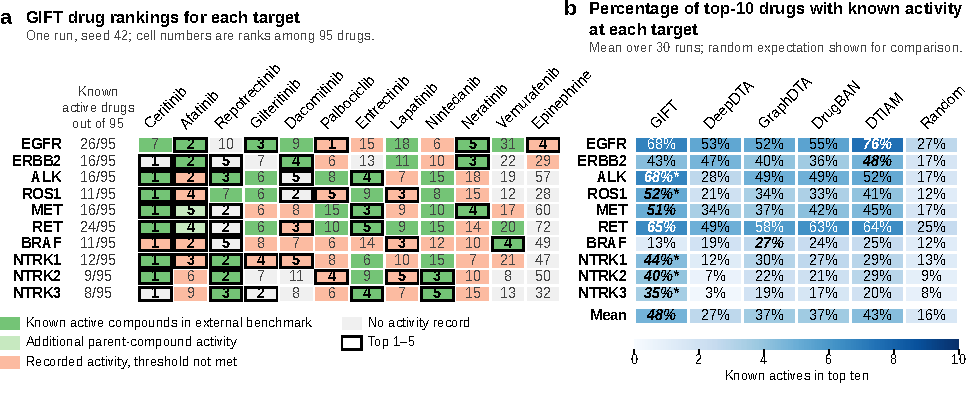
\includegraphics[width=\textwidth]{figs/lead_top_picks_gift.pdf}
\caption{Driver-kinase rankings of the 95 external drugs, with the kinases as shared rows. (a) Columns are the drugs ranked among the five highest for at least one kinase; outlined cells are the top 1-5, and colors give the evidence (known active: median pChEMBL $\geq5$ in ChEMBL~36; parent-compound activity: pChEMBL $\geq5$ in ChEMBL~37 for the parent compound only; threshold not met: records without pChEMBL $\geq5$). (b) Cells give the percentage of the ten highest-ranked drugs that are known actives, shaded by their number; bold italic marks the highest mean among the five methods in each row; Random is the expectation for a random ranking (known actives$/95$). $^{*}$GIFT above each baseline (two-sided paired Wilcoxon test, Holm-corrected over the 40 kinase-baseline comparisons, $p<0.05$).}
\label{fig:toppicks}
\end{figure}

%
\section{Discussion}
\label{sec:discussion}
This study supports two findings. First, for DTI prediction, GIFT made the most precise predictions of all nine methods on all three benchmarks over 30 runs, and its margin over baselines trained on the same interactions, negatives, and validation set grew with task difficulty. Second, for compound prioritization, it enriched known actives among the top-ranked clinical-stage drugs outside the training graph, though for the driver kinases this enrichment is largely shared across the kinase family. A matched decomposition attributes these improvements to the inductive architecture, that is, the fusion classifier trained with node masking and the edge-aware encoder, rather than to the contrastive pretraining or the soft-edge module (Appendix~\ref{S-sec:attribution}).


Of these, the inductive fusion classifier accounts for most of the improvement in target identification: added to a matched standard GCN, it raises the compound-matched MCC from 0.27 to 0.54, higher in all 30 runs. By combining graph embeddings with descriptor encodings, the same model scores compounds without known interactions, including the external drugs, on which the standard GNNs fall to near-chance MCC (0.012 to 0.057). Its predictions are stable across runs (compound-matched MCC standard deviation 0.038, compared with 0.059 to 0.102 for the DTI models trained from scratch) and precise: baselines with higher recall obtain it by predicting many more pairs as interactions, whereas GIFT has the highest precision on all three benchmarks and makes 41\%, 38\%, and 22\% fewer total errors than the next-best method.


The edge-aware encoder, in turn, makes graph information usable for compounds outside the graph: where a matched standard GCN with the same fusion classifier degrades the external predictions, it raises the external MCC from 0.19 to 0.34, higher in all 30 runs. End-to-end fine-tuning in Phase~3b improves further on Phase~3a (compound-matched MCC 0.52 to 0.56; Appendix~\ref{S-sec:attribution}). Ablations of the training recipe under identical settings (Appendix~\ref{S-sec:ablation_phases}) show that node masking improves the external MCC (0.342 compared with 0.326, $p=0.04$, uncorrected), and that the contrastive pretraining of Phases~1 and~2 is not required for these results: starting from a random encoder leaves the MCC and the driver-kinase shortlist unchanged and raises the external ROC-AUC (0.760 compared with 0.725). We attribute the performance to the edge-aware encoder trained with the supervised masked procedure; the contrastive phases supply the soft-edge module and its proposals. The graph embeddings add recall of the actives of new compounds to the descriptor encoders (0.245 compared with 0.217) and a higher external MCC (0.342 compared with 0.327).

In all 30 runs and for every method, no validation or test interaction enters the message-passing graph, no test interaction is used for model selection, and negatives are sampled without access to held-out labels (Appendix~\ref{S-sec:robustness}); node features derive from chemical structure and protein sequence alone. Random-negative benchmarks alone overstate how well DTI models identify the targets of a compound \cite{pahikkala2015toward}: with compound-matched negatives, the MCC of the random forest falls from 0.512 to 0.095 and that of the best standard GNN from 0.634 to 0.268, whereas GIFT retains an MCC of 0.564. The comparison is not an artifact of these choices: it holds on test interactions alone, against negatives restricted to measured below-threshold pairs, at activity thresholds of pChEMBL 6 and 7, for positives with direct single-protein measurements, across compound-similarity strata, on interactions first reported after ChEMBL~35, and when the sequence baselines are retrained with their kinase domains retained (Appendices~\ref{S-sec:attribution} and~\ref{S-sec:robustness}).

Learning from the interaction graph also proves more effective than large-scale pretraining. DTIAM poses the strongest challenge among the baselines: its compound encoder is pretrained on 1.59 million ChEMBL molecules, which include 45 of the 95 external drugs, and its protein encoder (ESM-2) on millions of UniRef sequences, an advantage on the drugs outside our graph. GIFT, trained on only about 2,000 interactions per run, nevertheless exceeds it in PR-AUC, precision, MCC, and ROC-AUC on every benchmark in all 30 runs (external MCC 0.342 compared with 0.198; compound-matched MCC 0.564 compared with 0.199) and in both driver-kinase shortlist metrics (rank one 6.7 compared with 4.4; top 10 47.9 compared with 43.0). DTIAM reaches its high recall by predicting most pairs as interactions, with 17.8 times as many false positives on the external drugs. Large-scale pretraining therefore does not replace what GIFT learns from the interaction graph: which proteins a compound acts on.


Beyond aggregate metrics, the rankings recover approved kinase inhibitors. As GIFT scores compounds absent from the graph, it ranks clinical-stage drugs against proteins represented in the training graph without retraining. Its rankings recover clinically relevant pairs for treating lung cancer: ceritinib is ranked first for ALK in 28 of the 30 runs and dacomitinib is among the 10 top-ranked drugs for EGFR in 29 (Figure~\ref{fig:toppicks}a), consistent with their use in ALK- and EGFR-driven non-small cell lung cancer. The architecture is not disease-specific and can be trained on interaction data from other diseases, providing a general framework for prioritizing candidates for experimental testing.

The auxiliary soft-edge module plays a smaller role. It learns structure on a heterogeneous DTI graph without direct label supervision; in a third of the runs, its top compound-protein proposals recover held-out interactions at up to 8.5 times the chance rate. In a matched comparison (Table~\ref{S-tab:ablation42}), it leaves DTI prediction unchanged and slightly increases the number of driver kinases with a known active ranked first (6.7, compared with 6.3 for a matched random augmentation and 6.0 without soft edges).

This study has limitations. Negatives are untested rather than confirmed inactive pairs, so the reported precision is conservative. A descriptor-only variant of the same classifier ranks the external drugs comparably (Appendix~\ref{S-sec:attribution}), so the measured benefit of the graph for compounds outside it lies mainly in recall of their actives. GIFT performs best on well-characterized targets and kinases, including all ten driver kinases, and declines for sparsely characterized and non-kinase targets (external ROC-AUC 0.715 for kinases and 0.697 for the best-covered third of targets, compared with 0.578 and 0.515; Appendix~\ref{S-sec:generalization}); for the driver kinases, it reliably identifies kinase inhibitors but only partly captures their selectivity for individual kinases (Appendix~\ref{S-sec:attribution}). The demonstrated utility is therefore strongest for kinases; since the architecture is not specific to a target class or disease, extending it to other target classes, for example with richer protein representations or additional interaction data, is a natural direction for future work. Transfer beyond lung cancer remains to be tested, and the untested top-ranked candidates await experimental validation.

\section{Conclusion}
\label{sec:conclusion}
This work presented GIFT, a graph-based framework for DTI prediction and compound prioritization in lung cancer, combining an edge-aware GNN encoder and an inductive fusion classifier that applies to compounds without known interactions, with an auxiliary soft-edge module that proposes edges during representation learning. For DTI prediction, under a protocol in which no held-out interaction is visible in the message-passing graph, GIFT achieved the highest PR-AUC, precision, and MCC and the fewest errors of the nine evaluated methods on all three benchmarks, with an MCC of 0.818 on held-out ChEMBL~35 interactions, 0.564 in target identification, and 0.342 on drugs outside the training graph, compared with at most 0.723, 0.470, and 0.231 for the baselines, including a pretrained baseline. For compound prioritization, it ranked these drugs for each target with a mean per-target ROC-AUC of 0.689 over 252 targets and 0.780 over the ten driver kinases of non-small cell lung cancer, and it placed 3.1 times as many known actives among its 10 top-ranked candidates for these kinases as expected at random.
By recovering established lung cancer drug-target relationships and enriching candidate lists for kinase-active compounds, GIFT connects interaction prediction with biologically grounded compound prioritization. These findings support its use to identify compounds outside the training graph for focused experimental follow-up in lung cancer research.

\section*{Data and Code Availability}
The knowledge graph, the external evaluation set, and the code to reproduce every result are available at \repourl.

\section*{Acknowledgements}
We thank the Biomedical Machine Learning (BioML) group at Microsoft Research and members of the broader Microsoft Research community for thoughtful suggestions and useful conversations for this project.

\bibliographystyle{unsrt}
\bibliography{mybib}

\end{document}
